\subsection{研修间预约模块}  % todo subsub

\subsubsection{代码框架及分析}

此部分代码位于 \texttt{src/studyroom/} 中。

\begin{figure}[H]
    \centering
    \resizebox{\textwidth}{!}{
        \begin{minipage}[H]{0.5\textwidth}
            \centering
            \begin{forest}
                for tree={
                    grow=east,
                    draw,
                    edge={-latex},
                    rounded corners,
                    node options={align=center},
                    anchor=west,
                    parent anchor=east,
                    child anchor=west,
                    delay={where content={}{shape=coordinate}{}} % 避免错误节点
                }
                [root
                [src
                [studyroom
                [\_\_init\_\_.py]
                [available.py]
                [query.py]
                [reserve.py]
                ]
                ]
                [tests
                [test\_studyroom
                [available.py]
                [query.py]
                [reserve.py]
                ]
                ]
                ]
            \end{forest}
        \end{minipage}

        \hspace{0.8cm}

        \begin{minipage}[H]{0.45\textwidth}
            \raggedright
            \textbf{模块说明:}\\
            \vspace{0.2cm}
            \textbf{Query (\texttt{query.py})}\\
            该模块仅实现对 \texttt{url} 的简单请求,不作任何数据处理。它通过相应的 API 获取研修室的可用性和详细信息。\\
            \vspace{0.4cm}

            \textbf{Available (\texttt{available.py})}\\
            \texttt{available.py} 模块负责处理房间可用性数据。它分析当前和已预订的时间段,确定研修室可预约的时间段。\\
            \vspace{0.4cm}

            \textbf{Reserve (\texttt{reserve.py})}\\
            \texttt{reserve.py} 模块管理预约流程。它包括进行预约、检查预约状态以及在特定条件下自动取消预约的功能。
        \end{minipage}
    }
    \caption{研修间的目录结构及模块说明}
    \label{fig:directory_structure}
\end{figure}

\subsubsection{研修间预约实现原理}

华东师范大学研修间预约最少预约时长在 60 分钟以上,采用贪心思想,我们尽量预约更长的时间段以供使用,即使不能使用还可以及时离开。

查看研修间的预约情况,我们首先需要计算出可用时间都有哪些:

\begin{figure}[H]
    \centering
    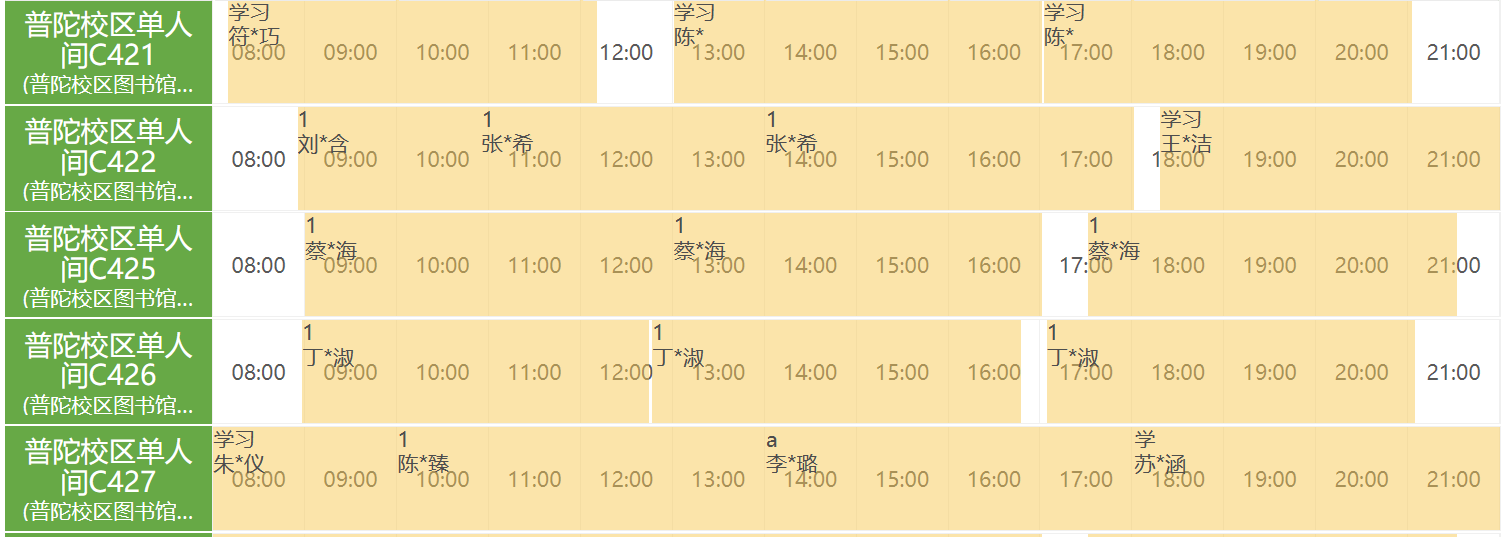
\includegraphics[width=0.62\textwidth]{img/studyroom_state.png}
    \caption{研修间状态示例}
    \label{fig:studyroom_available}
\end{figure}

研修间预约时,需要提交的表单样式如下,我们不采用浏览器自动操作的形式,而是截取提交时发送的 url 请求:

\begin{figure}[H]
    \centering
    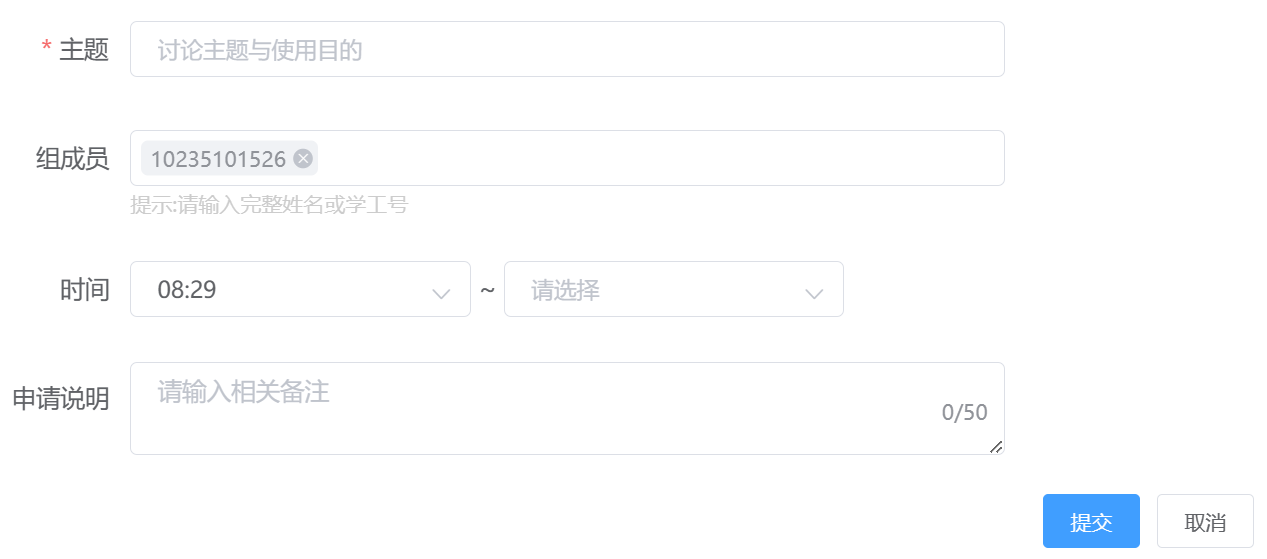
\includegraphics[width=0.5\textwidth]{img/studyroom_submit.png}
    \caption{研修间预约表单}
    \label{fig:studyroom_reserve}
\end{figure}

抓包得到 POST 请求的 Url 如下:\href{https://studyroom.ecnu.edu.cn/ic-web/reserve}{\underline{https://studyroom.ecnu.edu.cn/ic-web/reserve}}

只需传入相关的字段即可:

\begin{figure}[H]
    \centering
    \begin{minipage}[H]{0.45\textwidth} % 左侧放图片
        \centering
        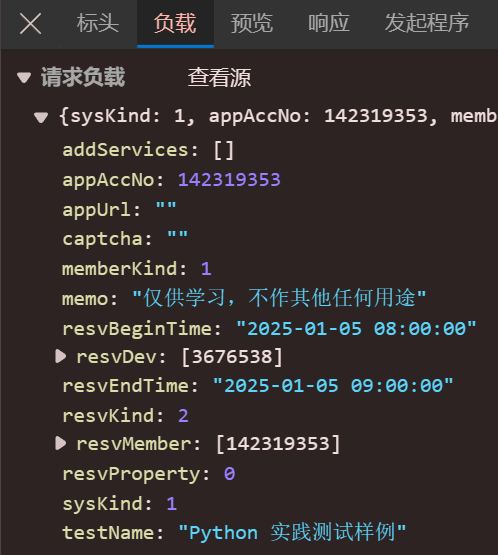
\includegraphics[width=0.6\textwidth]{img/studyroom_request.png}
        \caption{研修间预约请求}
        \label{fig:studyroom_request}
    \end{minipage}
    \hspace{0.05\textwidth} % 图片和代码之间的间距
    \begin{minipage}[H]{0.4\textwidth} % 右侧放代码
        \centering
        \begin{lstlisting}[language=python, caption={预约请求需要传入的字段}, label={lst:studyroom_request}]
headers = {
    "Cookie": f"ic-cookie={ic_cookie}", 
} # 从 StudyroomCache 中获取 ic-cookie

# 从 _fetch_userInfo 获取用户 ID
appAccNo = self._fetch_userInfo().get("accNo")

payload = {
    "sysKind": 1,  # 系统类型,默认为 1
    "appAccNo": appAccNo,
    "memberKind": 1,  # 成员类型,默认为 1
    "resvBeginTime": resvBeginTime,
    "resvEndTime": resvEndTime,
    "testName": testName,
    "resvMember": [appAccNo],
    # 默认预约人员列表只有当前用户
    "resvDev": resvDev,
    "memo": memo,
}
        \end{lstlisting}
    \end{minipage}
\end{figure}

加载入网页时,我们抓包发现,URL:\href{https://studyroom.ecnu.edu.cn/ic-web/roomDevice/roomAvailable}{\underline{URL: https://studyroom.ecnu.edu.cn/ic-web/roomDevice/roomAvailable}}
拥有查询当前类别的研修间的功能,其返回的字段如下:

\begin{lstlisting}[language=python]
    {'devId': 3676503,                             # 设备 ID
    'devName': '普陀校区单人间C421',                # 设备名称
    'minResvTime': 60,                             # 最小预约时间
    'openTimes': [{'openEndTime': '22:00',         # 开放结束时间
                   'openLimit': 1,                 # 最少预约人数
                   'openStartTime': '08:00'}],     # 开放开始时间
    'resvInfos': [{'resvBeginTime': '2024-12-26 '  # (People No.1) 的预约信息
                                    '17:01:00',
                   'resvEndTime': '2024-12-26 '
                                  '21:01:00',
                   'resvStatus': 1093}]},
\end{lstlisting}

它只为我们提供了 \texttt{'resvInfos'} 字段,这应该是用于前端供渲染黄色已预定时间段的给用户的,
所以我们需要将它与 \texttt{'openTimes'} 字段结合起来,得到研修室的可用时间段。

\begin{note}
    \begin{itemize}
        \item 将 [openStartTime, currentTime] 区间视为不可用时间段。例如当天 18:55 P.M 前的时间段都无效。
        \item 仅 AvailableTime > minResvTime 时,才将这段区间设置为 AvailableTime, 如果不超过最小预约时间,则不予考虑。
    \end{itemize}
\end{note}

返回的信息字典中,我们通过程序包含了一个新字段 \texttt{availableInfos},这样就可以提供给用户可用的时间段了。

之后,使用 \texttt{reserve.py} 中的函数 \texttt{\_fetch\_userInfo} 来获取 \texttt{appAccNo},这是识别用户身份的字段,
在发送 \texttt{reserve} 请求时,需要传入该字段作为 Payload 的一部分。最后通过调用 \texttt{reserve\_room} 函数即可完成全自动预约。

\begin{note}
    每一次预约都会形成一个唯一的预约编号,称为 \texttt{uuid},我们在进入个人中心时,网页会自动调用查询的接口:

    \href{https://studyroom.ecnu.edu.cn/#/ic/userinfo}{\underline{https://studyroom.ecnu.edu.cn/\#/ic/userinfo}}
    ,所以,我们也可以通过抓包获取 uuid,便可以知道用户当前是否有预约了,这为后续的自动取消预约提供了保障。
\end{note}
